% !TeX program = xelatex

\documentclass[12pt]{article}

\usepackage{amsmath,amsthm,amsfonts,amssymb,amscd}
\usepackage{multirow,booktabs}
\usepackage[table]{xcolor}
\usepackage{fullpage}
\usepackage{lastpage}
\usepackage{enumitem}
\usepackage{fancyhdr}
\usepackage{mathrsfs}
\usepackage{wrapfig}
\usepackage{setspace}
\usepackage{calc}
\usepackage{multicol}
\usepackage{cancel}
\usepackage[title]{appendix}
\usepackage[retainorgcmds]{IEEEtrantools}
\usepackage[margin=1in]{geometry}
\usepackage{empheq}
\usepackage{framed}
\usepackage[most]{tcolorbox}
\usepackage[notlof,notlot,nottoc]{tocbibind}
\usepackage{graphicx}
% 中文
\usepackage{xeCJK}
\setCJKmainfont{Microsoft JhengHei}
\XeTeXlinebreaklocale "zh"
\XeTeXlinebreakskip = 0pt plus 1pt

\colorlet{shadecolor}{orange!15}

\setlength{\parindent}{0pt}
\setlength{\parskip}{1em}

% Theorem, Lemma, Proposition: italic
\theoremstyle{plain}
\newtheorem{theorem}{Theorem}
\newtheorem{lemma}[theorem]{Lemma}
\newtheorem{corollary}[theorem]{Corollary}
\newtheorem{proposition}[theorem]{Proposition}

% Definition, Exercise, Solution: normal font
\theoremstyle{definition}
\newtheorem*{definition}{Definition}
\newtheorem*{exercise}{Exercise}
\newtheorem*{solution}{Solution}
\newtheorem{example}[theorem]{Example}

% Remark
\theoremstyle{remark}
\newtheorem*{remark}{Remark}
\newtheorem{notation}{Notation}

\DeclareMathOperator{\sign}{sign}

\numberwithin{equation}{section}
\numberwithin{theorem}{section}

\begin{document}

\begin{titlepage}
    \centering

    \vspace*{4cm}

    {\Huge\bfseries
    Solution Manual of Probability
    \par}

    \vfill

    {\large
    \today
    \par}

\end{titlepage}

\setcounter{section}{0}

\begin{center}
{\LARGE \bfseries Chapter 2 in \cite{Hog10}}
\end{center}

\begin{exercise}[2.1-7]
    Let a random experiment be the casting of a pair of unbiased six-sided dice, 
    and let $X$ equal the smaller of the outcomes if they are different and the common 
    value if they are equal.
    \begin{enumerate}
    \item With reasonable assumptions, find the p.m.f. of $X$.
    \item Let $Y$ equal the range of the two outcomes (i.e. the absolute value of the difference
     of the largest and the smallest outcomes). Determine the p.m.f. $g(y)$ of $Y$ for $y=0, 1, 2, 3, 4, 5$.
    \end{enumerate}
\end{exercise}

\begin{solution}
題目表示出$X$是六面骰骰兩次中最小點數的隨機變數。因為合計有36種可能狀況，其中
可以知道數字為1的情況有11種，以此類推。更具體一點為，考慮$X=x$，那麼我們可以將 
\[
P(X\geq x)-P(X\geq x+1)=P(X=x)
\]
用來計算，因此
\[
(7-x)^2-(6-x)^2=13-2x
\]
所以$X$的p.m.f.為
\[
\frac{13-2x}{36}
\]

而$Y$的p.m.f.則可以直接計數(暫時沒想到其他辦法)得到
\[P(Y=y)=\begin{cases}
\frac{1}{6},\ y=0,\\
\frac{6-y}{18},\ y=1,2,3,4,5.
\end{cases}\]
\qed
\end{solution}

%%%%%%%%%%%%%%%%%%%%%%%%%%%%%%%%%%%%%%%%%%%

\begin{exercise}[2.1-11]
    In a lot (collection) of $100$ light bulbs, there are $5$ bad bulbs. An inspector
    inspects $10$ bulbs selected at random. Find the probability of finding at least 
    one defective bulb. Hint: First compute the probability of finding no defectives in 
    the sample.
\end{exercise}
\begin{solution}
    抽$10$個至少壞$1$個的機率
    $$
    P=1-\text{全部都是好的機率}=1-P'
    $$
    全部是好的機率就很好算了。
    $$
    P'=\frac{95}{100}\times\frac{94}{99}\cdots\times\frac{86}{91}
    $$
    藉由計算機，
    $$
    P=0.4163
    $$
    \qed
\end{solution}
%%%%%%%%%%%%%%%%%%%%%%%%%%%%%%%%%%%%%%%%%%%

\begin{exercise}[2.1-13]
    Let X be the no. of accidents per week in a factory. Let the p.m.f.
    of $X$ be
    $$
    f(x)=\frac{1}{(x+1)(x+2)},\quad x=0,1,2,\cdots.
    $$
    Find the conditional probability of $X\geq4$, given that $X\geq1$.
    Hint:Write $f(x)=1/(x+1)-1/(x+2)$.
\end{exercise}
\begin{solution}
    $$
    P(X\geq4|X\geq1)=\frac{P(X\geq4\cap X\geq1)}{P(X\geq1)}=\frac{P(X\geq4)}{P(X\geq1)}
    $$
    那麼先算$X\geq4$，
    $$
    P(X\geq4)=\sum^\infty_4 \frac{1}{n+1}-\frac{1}{n+2}=\frac{1}{5}
    $$
    以及
    $$
    P(X\geq1)=\sum^\infty_1 \frac{1}{n+1}-\frac{1}{n+2}=\frac{1}{5}=\frac{1}{2}
    $$
    所以答案為$\frac{2}{5}$。
    \qed
\end{solution}
%%%%%%%%%%%%%%%%%%%%%%%%%%%%%%%%%%%%%%%%%%%
\begin{exercise}[2.1-15]
    A professor gave her students six essay questions, from which she will select three for a test. A students has time to study for only three of these questions. 
    What is the probability that, of the questions studied,
    \begin{enumerate}
        \item at least one is selected for the test?
        \item all three are selected for the test?
        \item exactly two are selected for the test?
    \end{enumerate}
\end{exercise}
\begin{solution}
    教授挑選題目的種類為 $C^6_3=20$。
\begin{enumerate}
    \item 機率為1減掉全部都沒中的機率。全部都沒中的機率為
    $$
    \frac{20}{20\times 20}=\frac{1}{20}
    $$
    所以至少有一個被選中的機率為
    $$
    1-\frac{1}{20}=\frac{19}{20}
    $$
    \item 全部被選中的機率為
    $$
    \frac{20}{20\times 20}=\frac{1}{20}
    $$
    \item 恰好兩個被選中的機率為
    $$
    \frac{C^6_2\times C^4_1\times C^3_1}{20 \times 20}=\frac{180}{400}=\frac{9}{20}
    $$
\end{enumerate}
    \qed
\end{solution}
%%%%%%%%%%%%%%%%%%%%%%%%%%%%%%%%%%%%%%%%%%%
%%%%%%%%%%%%%%%%%%%%%%%%%%%%%%%%%%%%%%%%%%%
\begin{exercise}[2.1-17]
    Five card are selected at random without replacement from a standard, thoroughly shuffled 52-card deck of playing cards. 
    Let $X$ be the number of face cards (kings, queens, jacks) in the hand. Forty observations of $X$ yielded the following data:
    \begin{table}[h!]
    \begin{center}
    \begin{tabular}{*{20}{c}}
    2 & 1 & 2 & 1 & 0 & 0 & 1 & 0 & 1 & 1\\
    0 & 2 & 0 & 2 & 3 & 0 & 1 & 1 & 0 & 3\\
    1 & 2 & 0 & 2 & 0 & 2 & 0 & 1 & 0 & 1\\
    1 & 2 & 1 & 0 & 1 & 1 & 2 & 1 & 1 & 0
    \end{tabular}
    \end{center}
    \end{table}
    \begin{enumerate}
        \item Argue that the p.m.f. of $X$ is 
        $$
        f(x)=\frac{C^{12}_x\times C^{40}_{5-x}}{C^{52}_5},\quad x=0,1,2,3,4,5
        $$
        and thus, that $f(0)=2109/8330,f(1)=703/1666,f(2)=209/833,f(3)=55/833,f(4)=165/21658,f(5)=33/108290$.
        \item Draw a probability histogram for this distribution.
        \item Determine the relative frequencies of $0,1,2,3$, and superimpose the relative frequency histogram on your probability histogram.
    \end{enumerate}
\end{exercise}
\begin{solution}
\begin{enumerate}
    \item 分母沒有問題，分子左側為$12$人頭牌中剛好被拿出了幾張，以及非人頭牌被拿出剩下的張數。此分配為超幾何分配。
    \item 理論機率直方圖為 Figure~\ref{fig:1}。
    \begin{figure}[htbp]
    \centering
    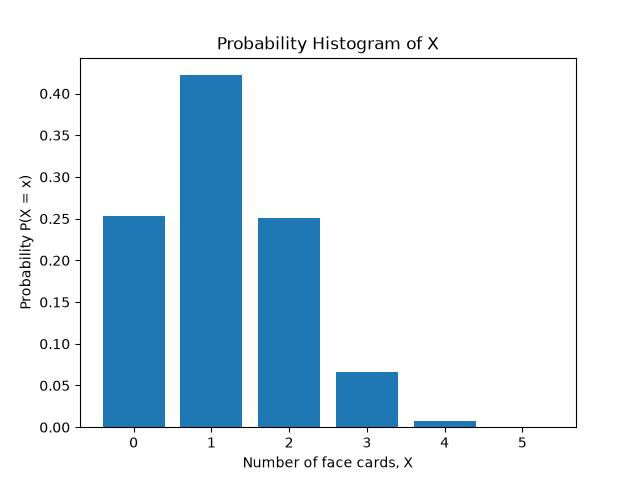
\includegraphics[width=0.5\textwidth]{img/Figure_1.jpeg} % 檔名與寬度設定
    \caption{理論機率直方圖} % 圖說
    \label{fig:1} % 標籤供交互參照
    \end{figure}
    \item 以「實驗得到的 relative frequency histogram」和「理論 probability histogram」比較 (Figure~\ref{fig:2})。能看出從實驗得到的數據與理論值雖有差異但還是相當接近。
    \begin{figure}[htbp]
    \centering
    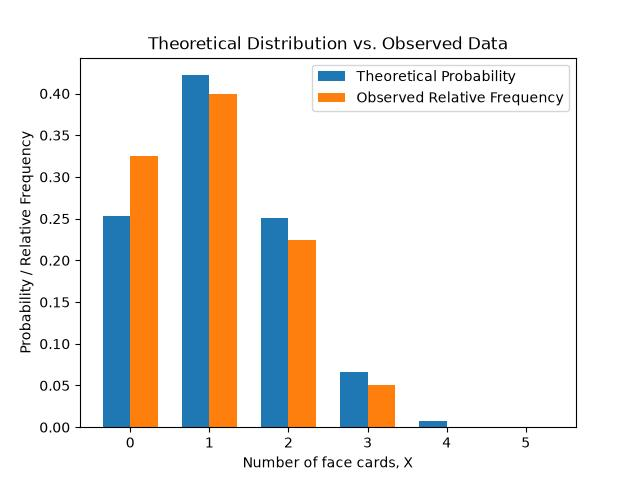
\includegraphics[width=0.5\textwidth]{img/Figure_2.jpeg} % 檔名與寬度設定
    \caption{相對機率直方圖} % 圖說
    \label{fig:2} % 標籤供交互參照
    \end{figure}
\end{enumerate}
    \qed
\end{solution}
%%%%%%%%%%%%%%%%%%%%%%%%%%%%%%%%%%%%%%%%%%%
\begin{exercise}[2.1-19]
    A bag contains 144 ping-pong balls. More than half of the balls are painted orange and the rest are painted orange and the rest are painted blue. Two balls are simultaneously drawn at random.
     The probability of drawing two balls of the same color is the same as the probability of drawing two balls of different colors. How many orange balls are in the bag?
\end{exercise}
\begin{solution}
假設橘球數量為$x$，從抽出同色與抽出異色機率相等出手，
$$
P(\text{同色})=P(\text{異色})
$$
分母都相同，分子列式為
$$\begin{aligned}
C^x_1C^{144-x}_1&=C^x_2+C^{144-x}_2,\\
288x-2x^2&=x(x-1)+(144-x)(143-x),\\
x=78 &\lor x=66.
\end{aligned}$$
所以橘色球數量為$78$個。
\qed
\end{solution}
%%%%%%%%%%%%%%%%%%%%%%%%%%%%%%%%%%%%%%%%%%%
\begin{exercise}[2.2-3]
    In a particular lottery, 3 million tickets are sold each week for 50¢ apiece. Out of the 3 million tickets, 12,006 are drawn at random and without replacement 
    and awarded prizes: twelve thousand \$25 prizes, four \$ 10,000 prizes, one \$50,000 prize, and one \$200,000 prize. If you purchased a single ticket, what is the expected value 
    of this game to you?
\end{exercise}
\begin{solution}
中 \$25 的機率為 $\frac{12000}{3000000}$，中 \$10000 的機率為 $\frac{4}{3000000}$，中 \$50000 的機率為 $\frac{1}{3000000}$，中 \$200000 的機率為 $\frac{1}{3000000}$，賠\$0.5的機率為 $1$ 因為一定要付錢買樂透。
所以列式為

$$
\begin{aligned}
E(X)&=\frac{12000}{3000000}\times 25+\frac{4}{3000000}\times 10000+\frac{1}{3000000}\times 50000+\frac{1}{3000000}-\frac{1}{2}\\
&=\frac{590000}{30000000}-\frac{1}{2}=\frac{59}{300}-\frac{1}{2}\\
&=\frac{-91}{300}\approx -0.3033
\end{aligned}$$
\qed
\end{solution}
%%%%%%%%%%%%%%%%%%%%%%%%%%%%%%%%%%%%%%%%%%%


\newpage

\nocite{*}
\bibliographystyle{siam}
\bibliography{ref}

\end{document}